\graphicspath{{./figures}}

\section{Ground Station Antenna}
\subsection{Mechanical Considerations}

The existing antennna mount is shown in Figure \ref{fig:antennaMount}. Azimuthal and elevation stepper motors are connected directly through Gear A and B respectively. Gear A rotates the centre shaft to provide azimuthal steering, whereas Gear B rotates through Gear D and E to allow a change in elevation. The 
specifications in Table \ref{tab:mount_specifications} were realized.

\begin{table}[!htb]
  \centering
  \renewcommand{\arraystretch}{1.2}
  \begin{tabular}{ |c|c| }
  \hline
  \textbf{Component}        & \textbf{Specification}    \\
  \hline
  Motor         & 200 full steps (per 360 degrees) \\ \hline
  Gear A        & 15 teeth \\ \hline
  Gear B        & 20 teeth \\ \hline
  Gear C        & 60 teeth \\ \hline
  Gear D        & 92 inner teeth, 80 outer teeth \\ \hline
  Gear E        & 140 teeth (equivalent) \\ \hline
  \end{tabular}
  \caption{Mount Gear and Motor Specifications}
  \label{tab:mount_specifications}
\end{table}

The black plastic platform is triangular and has three mounting holes. The new ground station's antenna should therefore be mounted onto this platform. It is important to consider the forces/torques involved, as well as the stepper motor holding torques, in order to determine the maximum weight and acceptable form factor of the new antenna.

The azimuthal motor need not be considered, as all torques from the mount to its base are perpendicular to the central shaft, meaning it would only need to overcome static frictional forces to rotate the antenna, which are assumed to be negligible. The holding torque of the elevation motor, however, will constrain the antenna design. The holding torque of each motor is 0.25 Nm. The gearing ratio resulting from Gears B, D and E, results in an around 8x torque increase. This provides a holding torque of around 2 Nm at the pivot axle.

The centre of gravity of the antenna, as well as its weight, will affect the motor's ability to hold it in place. The horizontal distance between the pivot axle and the mount in the upright position is measured to be 40mm. Therefore, in the worst-case (when the mount is upright as in Figure \ref{fig:antennaMount}) a planar antenna could weigh up to $\frac{2}{(9.8 \times 0.04)} = \SI{5.1}{kg}$. In general, the "mass-distance" product of the antenna (mass times distance of centre of gravity from mount) should not be more than $\SI{0.2}{kg \cdot m}$. This should be strongly considered if a longer antenna is desired.

The physical dimensions of the antenna's ground plane is also constrained. A circular ground plane may make contact with the mount's base at low elevation angles (assuming the ground station itself is raised above the ground). When the mount is resting, this constraint is imposed when the ground plane first makes contact with the mount's base. For a circular ground plane, this is around $\SI{360}{mm}$ diameter at an elevation angle of around 35 degrees.

\subsection{Theoretical Design}
As discussed, the antenna should be capable of receiving from both the 405 MHz radiosonde link, as well as the custom LoRa-based link in the amateur radio band of 430 to 440 MHz. A helical antenna is suggested, for the following reasons:
\begin{itemize}
    \item Ability to increase gain arbitrarily by increasing the number of windings
    \item High fractional bandwidth of 56\%, which may allow for a smaller antenna than other antenna types
    \item Ease of manufacture
\end{itemize}

The centre frequency $f_c$ of the antenna should first be selected. With a fractional bandwidth of 56\%, the inequality $f_c \times (1 - \frac{0.56}{2}) < \SI{405}{MHz}$ must hold. This gives an upper bound on the centre frequency of 562.5 MHz. A minimum ground plane diameter of no smaller than $0.5 \lambda$ is recommended in \cite{textbook-antennaTheoryAnalysisDesign}, and $0.75 \lambda$ in \cite{textbook-helicalAntenna}. It is, however, probable that a ground plane as small as $0.5 \lambda$ will adversely affect the radiation pattern near the end of the specified bandwidth.

Assuming the larger ground plane recommendation, the resulting ground plane diameter is $0.75 \times \frac{3e8}{562.5e6} = \SI{400}{mm}$, which is larger than the mechanical size constraint. Neverthless, $f_c = \SI{550}{MHz}$ is chosen as the initial centre frequency for simulations. the ground plane will then be decreased in size appropriately (towards $G_\lambda = 0.5$ i.e. \SI{270}{mm}) and the results observed.

The design parameters for a helical antenna are $f_c$ (centre frequency), $n$ (number of turns), $S$ (the spacing between turns), $C$ (the circumference) and $G$ (the ground plane diameter). Design formulae are provided in \cite{textbook-antennaTheoryAnalysisDesign}, and have been modified below to use relative values instead of absolute ones (i.e. $S_\lambda$ and $C_\lambda$ instead of $S$ and $C$). Directivity, in dBi, is given by:
$$
D_0 = 10 \log(15 \cdot n S_\lambda \cdot C_\lambda)
$$

$C_\lambda$ is typically kept at 1.0, meaning the cirumference is equal to the operating wavelength. As mentioned, a gain of around 5 dBi is required. However, a 3 dB bandwidth drop is estimated nearer to 400 MHz since it as the edge of the operating band. Further, the effect of a smaller ground plane will likely decrease performance by an estimated minimum of at least 1 dB. Therefore, a centre-frequency gain greater than 8 dBi will be designed for. This will also move the system towards the 20 dBi link margin. For this gain, the $n S_\lambda$ product should equal around 0.45. Although the optimal value for $S_\lambda$ is 0.23 \cite{textbook-antennaTheoryAnalysisDesign}, smaller values have been quoted to work \cite{site-helicalCalculator} and are mechanically easier to construct. Therefore, $S_\lambda = 0.15$ is chosen, and finally, $n \geq 3$.

\subsection{Simulation Design}
Simulation of a helical antenna is well documented in literature, and therefore the parameters can be varied iteratively and integrated into the antenna design process. For this project, FEKO software is used. An initial model with the above parameters, a large ground plane ($G_\lambda \approx 1.0$), and a wire diameter of $\SI{2.5}{mm}$ (chosen due to availability) is simulated. The resulting radiation pattern at the centre frequency of $f = \SI{550}{MHz}$ is shown in Figure \ref{fig:helix1_pattern_550MHz}, with a maximum gain of around 9.5 dBi.

\begin{figure}[!htb]
  \centering
  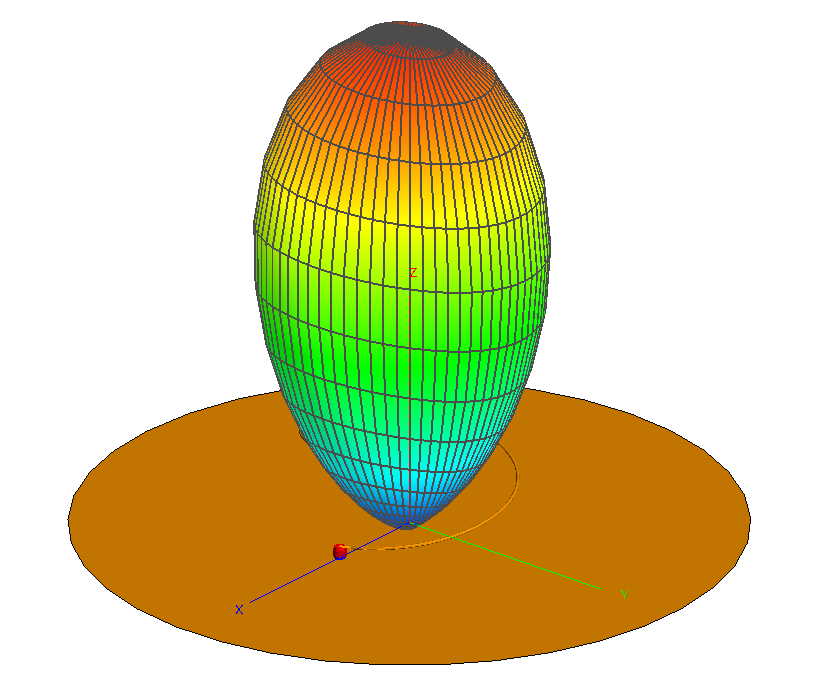
\includegraphics[width=0.45\textwidth]{helix1_pattern_550MHz}
  \caption{Initial Simulated Helical Antenna Radiation Pattern ($f=\SI{550}{MHz}$)}
  \label{fig:helix1_pattern_550MHz}
\end{figure}

Most of the follow-up design is conducted around the lower frequency of $f = \SI{405}{MHz}$. The radiation patterns for $G_\lambda = 0.5$ and $G_\lambda = 0.7$ ($G = \SI{273}{mm}$ and $G = \SI{382}{mm}$) are shown in Figures \ref{fig:helix2_pattern_405MHz} and \ref{fig:helix3_pattern_405MHz} respectively. It is clear that the recommended value of $G_\lambda = 0.5$ from \cite{textbook-antennaTheoryAnalysisDesign} will not work near this lower frequency, as shown by the morphed radiation pattern. The pattern is found to be acceptable at around $G_\lambda = 0.7$. However, after analysing the input impedance for this ground plane size (shown in Figure \ref{fig:helix3_impedance}) it is clear that broadband matching would be difficult, due to the drastic change in impedance near the lower end of the spectrum.

\begin{figure}[!htb]
  \begin{minipage}{.48\textwidth}
    \centering
    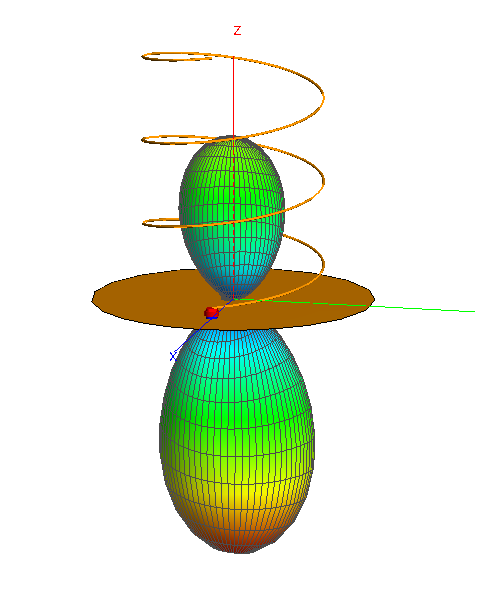
\includegraphics[width=0.6\linewidth]{helix2_pattern_405MHz}
    \caption{Simulated Helical Antenna Pattern at $f = \SI{405}{MHz}$ ($f_c = \SI{550}{MHz}$, $G_\lambda = 0.5$)}
    \label{fig:helix2_pattern_405MHz}
  \end{minipage}
  \begin{minipage}{.48\textwidth}
    \centering
    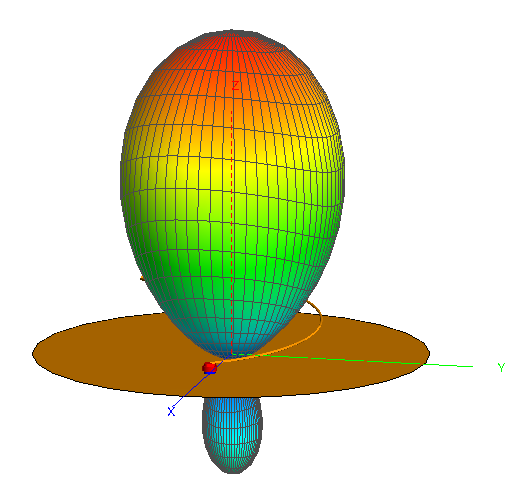
\includegraphics[width=0.75\linewidth]{helix3_pattern_405MHz}
    \caption{Simulated Helical Antenna Pattern at $f = \SI{405}{MHz}$ ($f_c = \SI{550}{MHz}$, $G_\lambda = 0.7$)}
    \label{fig:helix3_pattern_405MHz}
  \end{minipage}
\end{figure}

\begin{figure}[!htb]
  \centering
  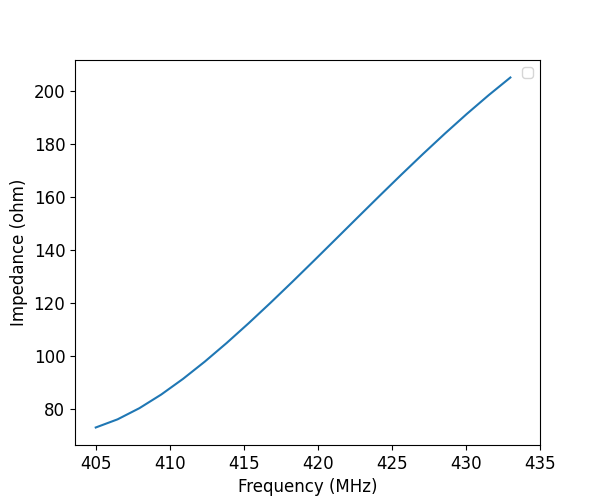
\includegraphics[width=0.65\textwidth]{helix3_impedance}
  \caption{Simulated Helical Antenna Input Impedance ($f_c = \SI{550}{MHz}$, $G_\lambda = 0.7$)}
  \label{fig:helix3_impedance}
\end{figure}

In order to ease matching, a lower centre frequency should ideally be used, to move the input impedance at 405 MHz and at 433 MHz closer together. This will, however, require either a larger ground plane, or a cupped ground plane (discussed further on). Unfortunately, FEKO does not allow for an optimisation goal that depends on two frequencies. Therefore, an iterative approach was used to find the centre frequency which minimizes the difference between the two impedances. The resulting centre frequency was found to be around $f_c = \SI{510}{MHz}$ at $G_\lambda = 0.6$ ($\approx \SI{350}{mm}$), with a resultant input impedance close to $\SI{250}{\ohm}$, as shown in Figure \ref{fig:helix4_impedance}.

\begin{figure}[!htb]
  \centering
  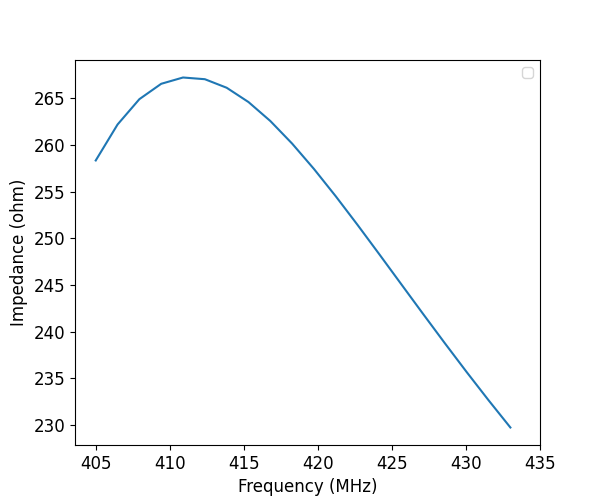
\includegraphics[width=0.65\textwidth]{helix4_impedance}
  \caption{Simulated Helical Antenna Input Impedance ($f_c = \SI{510}{MHz}$, $G_\lambda = 0.6$)}
  \label{fig:helix4_impedance}
\end{figure}

Since the mount can support a larger weight than the 3 turn coil, it was decided to experiment with larger a turn count (i.e. $n=4$), both for increased directivity/performance, and to potentially cater for manufacturing imperfections, such as a thin aluminium foil ground plane, and any diversions from the ideal helical shape. It was found that, for small ground plane diameters, as the number of turns increased, the radiation pattern for $f = \SI{405}{MHz}$ was negatively affected. This is intuitive when referring to image theory, as the non-idealities due to the finitely-sized ground plane become more apparent as distance to the plane increases. It should be noted that the pattern at $f = \SI{433}{MHz}$ was not as adversely affected.

The ground plane was therefore cupped, and the results observed. At $G_\lambda = 0.6$, a cup height equal to 1 helical turn was found to greatly improve the radiation pattern. This is shown in Figures \ref{fig:helix5_pattern_405MHz} and \ref{fig:helix6_pattern_405MHz}. The gain, however, was not as drastically affected.

\begin{figure}[!htb]
  \begin{minipage}{.49\textwidth}
    \centering
    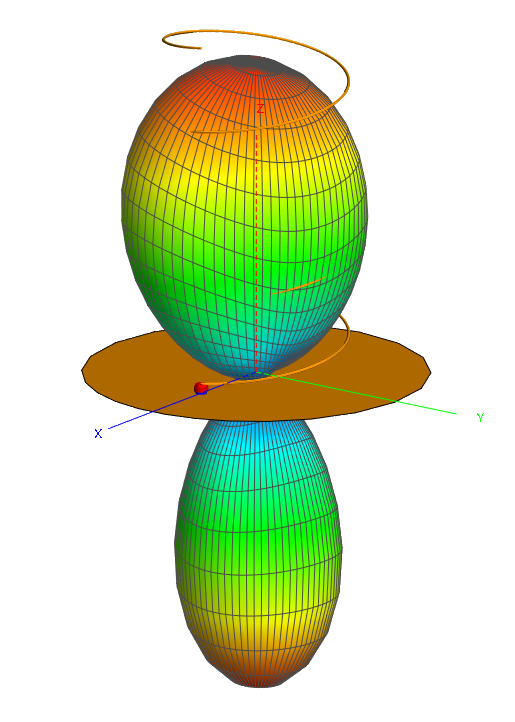
\includegraphics[width=0.5\linewidth]{helix5_pattern_405MHz}
    \caption{Simulated Helical Antenna Pattern without Cup ($G_\lambda = 0.6$, $f=\SI{405}{MHz}$)}
    \label{fig:helix5_pattern_405MHz}
  \end{minipage}
  \begin{minipage}{.49\textwidth}
    \centering
    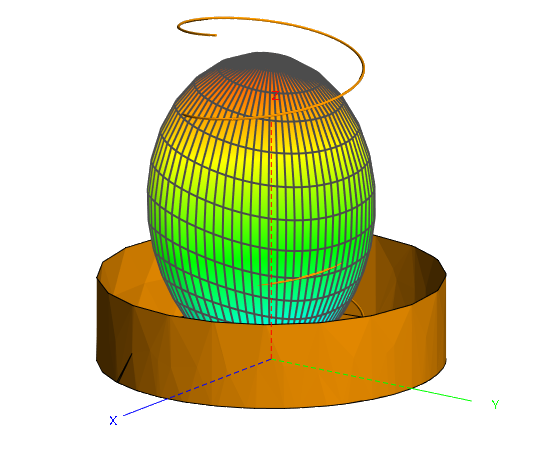
\includegraphics[width=0.85\linewidth]{helix6_pattern_405MHz}
    \caption{Simulated Helical Antenna Pattern with Cup ($G_\lambda = 0.6$, $f=\SI{405}{MHz}$)}
    \label{fig:helix6_pattern_405MHz}
  \end{minipage}
\end{figure}

It was therefore decided that the antenna would initially be built with a large ground plane and higher number of turns. Then, after measurement results and protocol implementation, the ground plane would be decreased appropriately to fit onto the mount. If time allows, and it is deemed necessary, a cup will then be added to the ground plane, to improve the pattern and antenna performance, and cater for the radiosonde link. The final model parameters are then $D = \SI{187.1}{mm}$, $S = \SI{88.2}{mm}$, $n = 4$, and $G = \SI{350}{mm}$.

\subsection{Matching}
Impedance matching should be done if the helical antenna is to be fed by a $\SI{50}{\ohm}$ coaxial cable. It was decided to match the antenna to the custom link's frequency of $f = \SI{433}{MHz}$ using the strip method mention in Section \ref{sec:helical_matching} for an uncupped ground plane. The FEKO model for this method is shown in Figure \ref{fig:helix7_model}.

\begin{figure}[!htb]
  \centering
  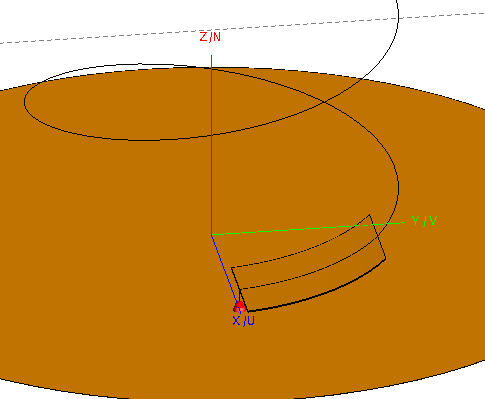
\includegraphics[width=0.45\textwidth]{helix7_model}
  \caption{Helical Antenna with Matching Strip Simulation Model}
  \label{fig:helix7_model}
\end{figure}

The strip is recommended to be relatively flat, and extend for approximately the first quarter turn. Its pitch angle was therefore chosen to be half that of the full helix, and it was chosen to extend for $0.15$ turns. The unknown parameters for the strip are then its height above the ground plane (also the height of the coaxial pin), and its strip width. The FEKO optimiser was used to optimise these two parameters for a minimum return loss. The resulting return loss as a function of frequency is shown in Figure \ref{fig:helix7_returnLoss}. The resultant mismatch loss is close to 0 dB at the target frequency, and 0.451 dB at 405 MHz.

\begin{figure}[!htb]
  \centering
  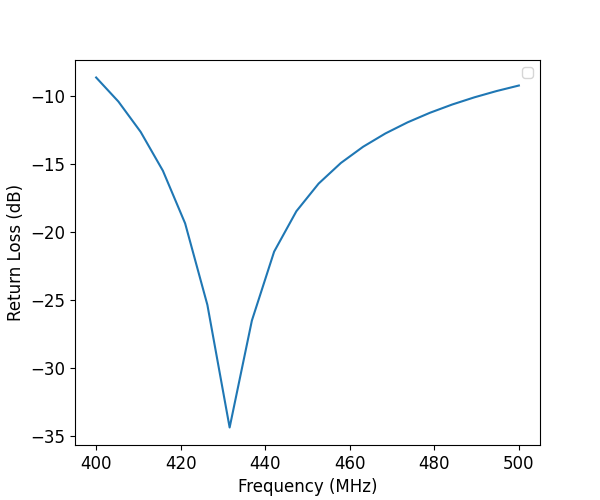
\includegraphics[width=0.85\textwidth]{helix7_returnLoss}
  \caption{Simulated Helical Antenna Return Loss vs Frequency}
  \label{fig:helix7_returnLoss}
\end{figure}

\newpage
The final antenna parameters are:
\begin{table}[!htb]
  \centering
  \renewcommand{\arraystretch}{1.2}
  \begin{tabular}{ |c|c| }
  \hline
  \textbf{Parameter}                  & \textbf{Value}    \\
  \hline
  Diameter (D)                        & 187.1 mm          \\ \hline
  Turn Spacing (S)                    & 88.2 mm           \\ \hline
  No. of Turns (n)                    & 4                 \\ \hline
  Ground plane diameter (G)           & $> \SI{350}{mm}$  \\ \hline
  Strip height (sh)                   & 19.4 mm          \\ \hline
  Strip width (sw)                    & 77.7 mm           \\ \hline
  Strip length (sl)                   & 132 mm           \\ \hline
  Cup height, if used (ch)            & 88.2 mm           \\ \hline
  \end{tabular}
  \caption{Helical Antenna Final Parameters}
  \label{tab:helicalParameters}
\end{table}